%!TEX root = report_template.tex

\documentclass{article}
\usepackage{CJKutf8}
\usepackage{graphicx}
\usepackage{enumerate}
\usepackage{amsmath}
\usepackage{amsthm}
\usepackage{amsfonts}
\usepackage{hyperref}
\usepackage{subfigure}
\usepackage{amsmath}  

\usepackage{geometry}
\geometry{left=3.5cm,right=3.5cm,top=4.0cm,bottom=4.0cm}
\usepackage{times}

\usepackage{indentfirst}

\usepackage{algorithm}  
\usepackage{algpseudocode}  
\usepackage{amsmath}  
\renewcommand{\algorithmicrequire}{\textbf{Input:}}  % Use Input in the format of Algorithm  
\renewcommand{\algorithmicensure}{\textbf{Output:}} % Use Output in the format of Algorithm    
\usepackage{listings}
\usepackage{url}

\usepackage{etoolbox}
\newtoggle{solution}
\toggletrue{solution}
% \togglefalse{solution}

\usepackage{color}
\usepackage[dvipsnames]{xcolor}
\newcommand{\solution}[2][0pt]{\iftoggle{solution}{\smallskip{\color{red}{\flushleft\textbf{Solution}:}\par#2}}{\vspace*{#1}}}

\renewcommand{\baselinestretch}{1.2}%Adjust Line Spacing
%\geometry{left=2.0cm,right=2.0cm,top=2.0cm,bottom=2.0cm}% Adjust Margins of the File

% Create horizontal rule command with an argument of height
\newcommand{\horrule}[1]{\rule{\linewidth}{#1}}
% Set the title here
\title{
    \normalfont \normalsize
    \large \textsc{ShanghaiTech University} \\ [15pt]
    \horrule{2pt} \\[0.5cm] % Thin top horizontal rule
    \huge CS271 Computer Graphics \uppercase\expandafter{\romannumeral 2} \\ % The assignment title
    \LARGE Fall 2025\\
    \LARGE Problem Set 1\\
    \horrule{2pt} \\[0.5cm] % Thick bottom horizontal rule
}
% wrong usage of \author, never mind
\author{}
\date{Due: 23:59, Oct. 24, 2025}

% Add the support for auto numbering
% use \problem{title} or \problem[number]{title} to add a new problem
% also \subproblem is supported, just use it like \subsection
\newcounter{ProblemCounter}
\newcounter{oldvalue}
\newcommand{\problem}[2][-1]{
	\setcounter{oldvalue}{\value{secnumdepth}}
	\setcounter{secnumdepth}{0}
	\ifnum#1>0
		\setcounter{ProblemCounter}{#1}
	\else
		\stepcounter{ProblemCounter}
	\fi
	\section{Problem \arabic{ProblemCounter}: #2}
	\setcounter{secnumdepth}{\value{oldvalue}}
}
\newcommand{\subproblem}[1]{
	\setcounter{oldvalue}{\value{section}}
	\setcounter{section}{\value{ProblemCounter}}
	\subsection{#1}
	\setcounter{section}{\value{oldvalue}}
}

\begin{document}
\maketitle
\vspace{3ex}

\begin{enumerate}
%\item Please write your solutions in English. 
\item Submit your \textcolor{blue}{\textbf{PDF}} solution to the course \textbf{Gradescope}. \textbf{[Code: 8XV4G8]}
\item Submit your \textcolor{blue}{\textbf{Source Code and PDF as a zip file}} to the \textbf{ShanghaiTech EPAN}:  \url{https://epan.shanghaitech.edu.cn/l/RF2KH8}. [\textbf{Filename:} \verb|name_2025xx(your id)_hw1.zip|]
% \item If you want to submit a handwritten version, scan it clearly.
\item There are no restrictions on programming languages.  
\item You are required to follow ShanghaiTech's academic honesty policies. You are allowed to discuss problems with other students, but you must write up your solutions by yourselves. You are not allowed to copy materials from other students or from online or published resources. Violating academic honesty can result in serious penalties.  
\end{enumerate}

\newpage
\problem{Melkman's Algorithm for Simple Polygon Convex Hull}

Implement Melkman's algorithm to compute the convex hull of a simple polygon in $\mathcal{O}(n)$ time complexity.\bigskip

\noindent \textbf{Reference:} Lecture 2, page 71

\noindent \textbf{Requirements:}
\begin{enumerate}
    \item \textbf{Input:} A simple polygon represented as an ordered sequence of $n$ vertices.
    \item \textbf{Output:} The convex hull vertices in counterclockwise order.
    \item Complexity analysis explaining why the algorithm achieves $\mathcal{O}(n)$ time.
    \item Test cases with at least three different polygons.
\end{enumerate}

\subsection*{1. Problem Definition and Notation}

\textbf{Simple polygon:} A simple polygon is a two-dimensional planar shape formed by connecting a finite sequence of distinct vertices in order and closing the loop. Adjacent edges meet only at their shared endpoints, and no non-adjacent edges intersect. This guarantees a single, connected, and non-self-intersecting boundary that encloses a finite region in the plane. In this report, we focus exclusively on polygons in the two-dimensional Euclidean space $\mathbb{R}^2$, since Melkman’s algorithm is specifically designed for 2D convex hull construction.

\textbf{Goal:} The goal of Melkman’s algorithm is to compute the convex hull of a simple polygon efficiently in linear time $\mathcal{O}(n)$. 
Given an ordered vertex sequence representing the boundary of a simple polygon, the algorithm constructs the smallest convex polygon that completely contains it, returning the convex hull vertices in counterclockwise order.

\textbf{Notation:} The input polygon is represented as an ordered vertex sequence $P = (p_0, p_1, \dots, p_{n-1})$, where each vertex $p_i = (x_i, y_i) \in \mathbb{R}^2$. 
Edges are implicitly defined between consecutive vertices $(p_i, p_{i+1})$ for $i = 0, 1, \dots, n-2$, and the polygon is closed conceptually by connecting $p_{n-1}$ back to $p_0$, without explicitly storing a duplicate vertex in the sequence. 
The output convex hull is denoted as $H = (h_0, h_1, \dots, h_{m-1})$. 
To evaluate geometric relations, the orientation of three points $a$, $b$, and $c$ is determined using the signed area function:
\[
\text{orient}(a,b,c) = (b_x - a_x)(c_y - a_y) - (b_y - a_y)(c_x - a_x),
\]
where a positive value means that $c$ lies to the left of the directed edge $ab$, a negative value indicates the right side, and zero denotes collinearity.

\subsection*{2. Data Structures and Algorithmic Idea}

\paragraph{2.1 Data structures}\

The input of the algorithm is an ordered list of vertices $P = (p_0, p_1, \dots, p_{n-1})$, where each vertex $p_i = (x_i, y_i) \in \mathbb{R}^2$ defines the boundary of a simple polygon. 
These vertices are accessed sequentially according to their order in $P$.

To maintain the evolving convex hull during the scan, the algorithm employs a double-ended queue $D$, which simultaneously stores the upper and lower hull chains. 
The front of $D$ corresponds to the starting point of the upper chain, while the back corresponds to the end of the lower chain. 
Each element of $D$ is a vertex from $P$, and the deque supports constant-time insertion and deletion operations at both ends:
\[
D = [d_0, d_1, \dots, d_k], \quad d_i \in P.
\]
This structure allows the algorithm to dynamically add or remove vertices when maintaining the left-turn property required for convexity. 
At the end of the iteration, the vertices remaining in $D$ form the convex hull in counterclockwise order.

\paragraph{2.2 Algorithmic idea}\

Melkman’s algorithm incrementally constructs the convex hull of a simple polygon in a single linear pass over its ordered vertices. 
It maintains a double-ended queue $D$ that simultaneously represents the upper and lower chains of the evolving convex hull. 
Initially, the algorithm identifies the first three non-collinear vertices $(p_0, p_1, p_2)$ and arranges them so that they form a counterclockwise triangle. 
These three vertices are inserted into the deque with $p_2$ appearing at both ends, establishing the initial convex structure.
For each subsequent vertex $p_i$ from the polygon, the algorithm tests whether $p_i$ lies inside the current hull defined by $D$. 
If the point is inside (to the left of both the top and bottom edges), it is skipped. 
Otherwise, $D$ is updated by removing points from the front and back that would cause the hull to turn right or become non-convex with respect to $p_i$. 
After pruning, $p_i$ is inserted at both ends, maintaining the counterclockwise convex boundary. 
This procedure ensures that each vertex is processed exactly once, and each is inserted and removed at most a constant number of times, leading to linear time complexity.

\begin{algorithm}[H]
\caption{Melkman’s Convex Hull for a Simple Polygon}
\begin{algorithmic}[1]
\Require Ordered vertices of a simple polygon $P = (p_0, p_1, \dots, p_{n-1})$
\Ensure Convex hull vertices $H$ in counterclockwise order

\State Initialize deque $D$ so that $p_0, p_1, p_2$ form a CCW triangle and $p_2$ appears at both ends:
\If{$\text{orient}(p_0, p_1, p_2) > 0$}
    \State Append in order: $p_2, p_0, p_1, p_2$
\Else
    \State Append in order: $p_2, p_1, p_0, p_2$
\EndIf

\For{$i = k+1$ to $n-1$}
    \State $p \gets p_i$
    \State $in\_top \gets \text{is\_left}(D[-2], D[-1], p)$
    \State $in\_bot \gets \text{is\_left}(D[0], D[1], p)$
    \If{$in\_top$ \textbf{and} $in\_bot$}
        \State \textbf{continue} \Comment{$p$ lies inside current hull}
    \EndIf

    \While{$\text{is\_right\_or\_on}(D[0], D[1], p)$}
        \State $D.\text{popleft}()$
    \EndWhile
    \State $D.\text{appendleft}(p)$

    \While{$\text{is\_right\_or\_on}(D[-2], D[-1], p)$}
        \State $D.\text{pop}()$
    \EndWhile
    \State $D.\text{append}(p)$
\EndFor

\State $D.\text{pop}()$ \Comment{Remove duplicated endpoint}
\State $H \gets$ list of vertices in $D$ (CCW order)
\State \Return $H$
\end{algorithmic}
\end{algorithm}

\subsection*{3. Test Case Design}

\paragraph{3.1 Special cases}\

To ensure the robustness and correctness of Melkman’s algorithm, several representative special cases are considered in the test design. 
First, polygons containing multiple nearly collinear vertices are used to evaluate numerical stability when the orientation value $\text{orient}(a,b,c)$ approaches zero. 
These cases verify that the algorithm correctly handles degenerate configurations and maintains consistent convexity. 

Second, polygons with concave indentations (pocket structures) are designed to test the deque’s bidirectional update mechanism. 
Such inputs trigger both front and back popping operations, ensuring that the convex hull update process preserves the counterclockwise convex boundary.

Third, near-contact configurations are introduced, where two non-adjacent edges approach each other closely without intersecting. 
These cases assess the algorithm’s tolerance to small geometric gaps and verify that floating-point precision errors do not lead to incorrect intersection or collinearity detection.

Fourth, polygons containing many interior points but few exterior ones are used to test the skip logic. 
Internal points should be efficiently identified and ignored, confirming that the algorithm retains its linear-time complexity $\mathcal{O}(n)$ even for dense inputs.

Finally, inputs with reversed (clockwise) vertex order are included to confirm that the algorithm correctly identifies orientation and still produces a valid counterclockwise convex hull. 
Together, these cases cover the most critical geometric and numerical challenges that can occur in two-dimensional convex hull computation for simple polygons.

\paragraph{3.2 Case 1: Collinear Band with Near-Degenerate Contact}\

\textbf{Objectives and algorithmic checks:}
\begin{enumerate}
    \item Test stability of orientation when many consecutive vertices are collinear or nearly collinear ($\text{orient}(a,b,c)\!\approx\!0$); confirm correct seed-triple discovery during initialization and a consistent collinearity policy that retains only extreme endpoints on collinear runs.
    \item Test numerical robustness on an extremely narrow-band polygon with very small local area; verify inside-tests on both chains remain stable at the precision limit.
    \item Test tolerance to near-contact without intersection; ensure deque updates are correct when the near-contact tip triggers repeated front/back popping, preserving convexity and preventing vertex loss.
\end{enumerate}

\textbf{Construction method:}
An upper horizontal band at $y=520$ is formed by a long collinear sequence from $[150,520]$ to $[850,520]$, enforcing repeated $\text{orient}=0$ evaluations. A parallel lower band at $y=505$, only 15 units below, creates a narrow strip that amplifies floating-point sensitivity. A sharp vertex at $[560,518]$ lies merely 2 pixels beneath the upper band, producing a near-contact tip that stresses intersection and collinearity handling during deque updates. A closing vertex at $[140,490]$ slightly tapers the shape to keep a small but nonzero area so the polygon remains valid.

\textbf{Conclusion:}
Case~1 efficiently combines collinearity, near-degenerate geometry, and near-contact configurations in a single test. 
It provides a comprehensive stress test for the initialization, inside-test, and deque-update mechanisms of Melkman’s algorithm, confirming both its numerical robustness and geometric consistency.

\paragraph{3.3 Case 2: Dual-Pocket Polygon for Deque Update Validation}\

\textbf{Objectives and algorithmic checks:}\

\begin{enumerate}
    \item Verify the correctness of Melkman’s bidirectional deque update mechanism by constructing a polygon that simultaneously triggers both front and back popping operations.
    \item Examine the algorithm’s behavior when processing multiple concave pockets, ensuring that each concave indentation is correctly handled without breaking the convexity of the maintained hull.
    \item Confirm that the polygon remains simple and correctly closed during the entire hull construction process, with no edge crossings or ordering errors after repeated deque updates.
\end{enumerate}

\textbf{Construction method:}
The polygon is designed with two concave pockets—one on each side—to induce dual-end updates in the deque. On the left side, vertices $[180,300]$, $[160,340]$, and $[140,290]$ form the \emph{front pocket}, which triggers popping operations at the head of the deque. On the right side, vertices $[860,480]$, $[850,450]$, and $[820,520]$ create the \emph{rear pocket}, enforcing pops from the tail. The middle section, spanning from $[600,540]$ to $[900,520]$, forms a wide convex region that connects the two pockets smoothly. The remaining vertices follow a gentle transition, ensuring the polygon remains simple and fully enclosed.

\textbf{Conclusion:}
Case~2 effectively tests the update logic of Melkman’s algorithm by forcing alternating front and back popping during hull maintenance. 
It provides clear visual evidence of how the deque dynamically adjusts to restore convexity after processing concave pockets, validating the correctness of the update order, stopping conditions, and overall hull integrity.

\paragraph{3.4 Case 3: Interior-Point Skipping and Sparse Expansion Test}\

\textbf{Objectives and algorithmic checks:}\

\begin{enumerate}
    \item Verify that Melkman’s algorithm correctly identifies interior points located within the current convex hull and efficiently skips them without affecting the boundary structure.
    \item Test the correctness of hull expansion when a few exterior vertices appear after long sequences of interior points, ensuring that convexity restoration occurs only when necessary.
    \item Evaluate the algorithm’s ability to maintain its linear-time complexity $\mathcal{O}(n)$ under mixed input conditions containing both dense interior and sparse exterior vertices.
\end{enumerate}

\textbf{Construction method:}
The polygon is composed of two contrasting regions: a dense interior section and a sparse outer shell. The outer hull is defined by vertices such as $[200,600] \rightarrow [780,610] \rightarrow [860,640]$ and $[180,180]$, forming a broad convex frame. Between these outer points lies a long internal sequence, e.g., $[820,400] \rightarrow [400,400] \rightarrow [220,300]$, where most vertices remain strictly inside the convex boundary. These interior runs are occasionally interrupted by a few exterior expansion points, forcing the deque to update selectively. The alternating distribution of interior and exterior vertices provides a realistic stress test for the skip logic and incremental hull growth.

\textbf{Conclusion:}
Case~3 demonstrates the efficiency of Melkman’s algorithm in distinguishing interior from exterior vertices and preserving its $\mathcal{O}(n)$ time behavior even for highly unbalanced input distributions. 
It confirms that unnecessary updates are avoided for interior points, while sparse exterior vertices correctly trigger localized deque modifications, maintaining a consistent and minimal convex hull.

\paragraph{3.5 Visual summary and case coverage}\  

\begin{figure}[H]
    \centering
    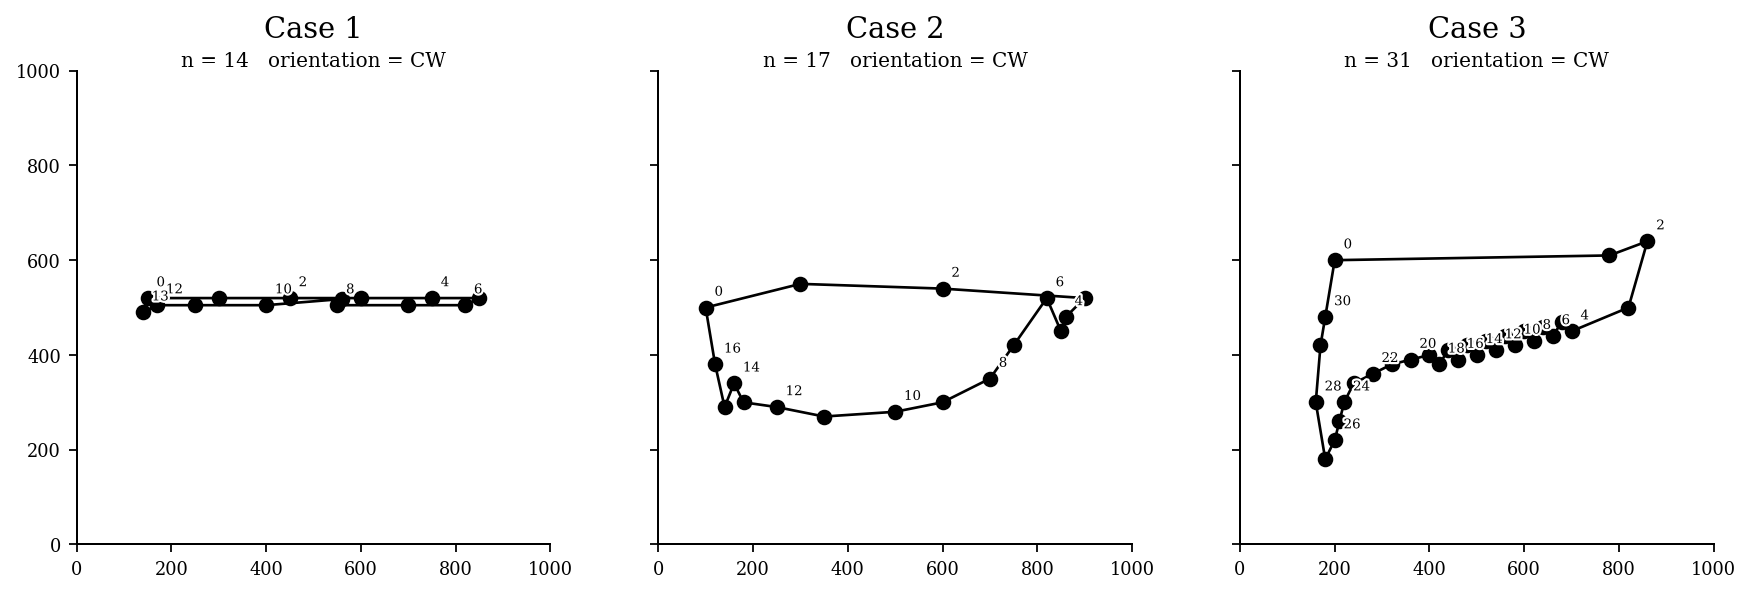
\includegraphics[width=0.9\linewidth]{Pictures/polygon_cases.png}
    \caption{Visualization of the three representative polygon cases used in testing Melkman’s algorithm. 
    Case~1: collinear band with near-degenerate contact; 
    Case~2: dual-pocket polygon; 
    Case~3: interior-point skipping with sparse expansion.}
\end{figure}

\textbf{Summary of coverage:}
The three designed cases jointly encompass the major geometric and numerical challenges identified in Section~3.1. 
Case~1 focuses on numerical stability under collinearity, near-degenerate geometry, and near-contact configurations, verifying that orientation, convexity, and initialization logic remain robust at precision limits. 
Case~2 targets the algorithm’s structural correctness during hull updates by introducing concave pockets that activate both front and back deque operations, testing update order and boundary integrity. 
Case~3 evaluates performance and correctness in mixed-density inputs, where numerous interior points are interleaved with sparse exterior ones, validating the skip logic and maintenance of linear-time behavior.

Together, these cases comprehensively test Melkman’s algorithm across initialization, inside-testing, and deque-update phases. 
They confirm that the implementation is robust to collinearity, concavity, and numerical perturbation, while preserving correctness and $\mathcal{O}(n)$ efficiency across all representative polygon configurations.

\subsection*{4. Visualization and Results Analysis}\

Following the design principles and definitions described in previous sections, the Melkman convex hull algorithm was implemented and tested on the three representative polygon cases defined in Section~3. 
The results are shown in Figure~\ref{fig:hulls}, where each subfigure corresponds to one of the test cases: 
Case~1 (collinear band with near-degenerate contact), 
Case~2 (dual-pocket polygon), 
and Case~3 (interior-point skipping and sparse expansion).

\begin{figure}[H]
    \centering
    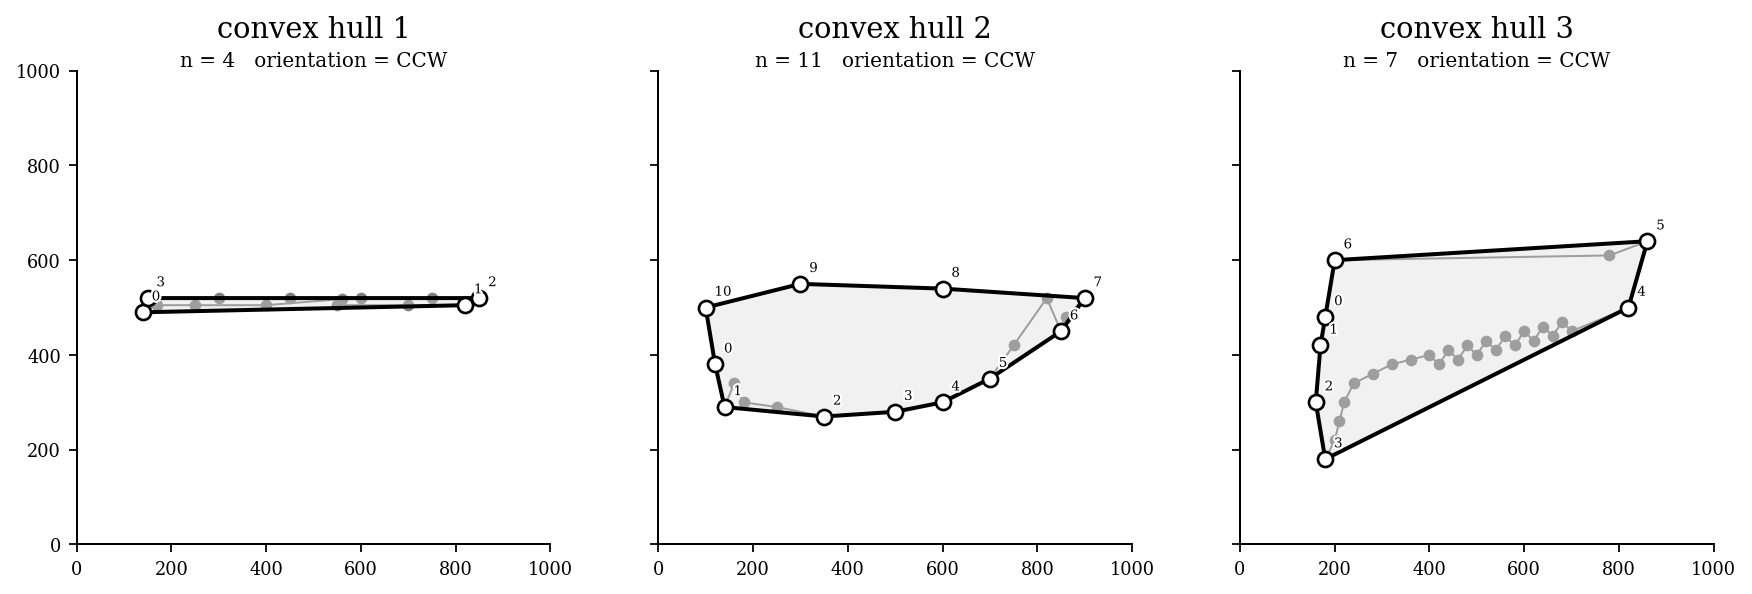
\includegraphics[width=0.95\linewidth]{Pictures/hulls.png}
    \caption{Visualization of convex hull results for the three designed test cases. 
    Each subfigure shows the original polygon (gray line and points) and the computed convex hull (bold black outline). 
    Hull vertices are labeled in counterclockwise order, and $n$ denotes the number of vertices in each polygon.}
    \label{fig:hulls}
\end{figure}

\textbf{Result correctness and analysis:}  
The visual outcomes confirm that Melkman’s algorithm produces the expected convex boundaries for all three input categories.

For \emph{Case~1}, only the extreme vertices of the upper and lower collinear bands are retained, while all intermediate collinear points are correctly excluded from the hull. 
The narrow-band configuration demonstrates stable orientation evaluation even when $\text{orient}(a,b,c) \approx 0$, indicating numerical robustness against near-degenerate geometry.

For \emph{Case~2}, the presence of two concave pockets successfully triggers deque updates at both ends. 
The hull reconstruction after each concave indentation preserves convexity and counterclockwise orientation, verifying the correctness of the bidirectional popping mechanism.

For \emph{Case~3}, the majority of interior points are efficiently skipped, while a few exterior vertices correctly expand the hull boundary. 
The algorithm maintains linear-time behavior since each vertex is processed at most once, confirming that the skip logic prevents redundant operations.

Overall, the visualization results align perfectly with the theoretical expectations. 
Melkman’s algorithm demonstrates robustness across numerical edge cases, correctness in deque-based updates. 
The generated convex hulls exhibit clean, non-intersecting boundaries that accurately enclose the input polygons.

\subsection*{5. Time Complexity Analysis}\

\paragraph{5.1 Theoretical}\

Melkman’s algorithm achieves linear-time complexity $\mathcal{O}(n)$ with respect to the number of vertices in the input polygon. 
The efficiency arises from its incremental and deterministic construction process, which guarantees that each vertex is handled a constant number of times. 

During the main loop, each vertex $p_i$ is read exactly once in the scanning order of the polygon. 
For each $p_i$, the algorithm performs a constant number of orientation tests and at most a few deque operations. 
Each vertex can be inserted into and removed from the deque at most once per end—once when it enters the convex hull and once when it is later popped due to a non-left turn. 
Therefore, the total number of deque operations over the entire run is proportional to $n$.

The orientation test $\text{orient}(a,b,c)$, which involves a few arithmetic operations on vertex coordinates, also executes $\mathcal{O}(1)$ per call. 
Even under degenerate cases such as long collinear sequences, each vertex still contributes only a bounded number of constant-time comparisons before either being skipped or becoming part of the hull.

As a result, the total computational cost can be expressed as:
\[
T(n) = c_1 n + c_2 n + c_3 n = \mathcal{O}(n),
\]
where $c_1$, $c_2$, and $c_3$ correspond to the constant-time costs of orientation evaluation, deque maintenance, and inside-testing respectively. 
No nested loops dependent on $n$ exist in the algorithm, and no vertex is ever revisited or reprocessed after being finalized in the hull. 

Hence, Melkman’s convex hull algorithm is theoretically proven to run in $\mathcal{O}(n)$ time for any simple polygon input, achieving optimal performance for this class of problems.

\paragraph{5.2 Empirical}\

To validate the theoretical time complexity, an experimental evaluation was conducted using a series of polygons with progressively increasing vertex counts. 
Nine polygon sets were generated to provide a controlled range of input sizes, ensuring both reproducibility and consistent geometric diversity. 
The generated polygons are visualized in Figure~\ref{fig:testpolys}, and their corresponding convex hulls, computed using the implemented Melkman algorithm, are shown in Figure~\ref{fig:testhulls}. 
Each convex hull result was visually verified to confirm correctness before performing timing and operation-count measurements.

\begin{figure}[H]
    \centering
    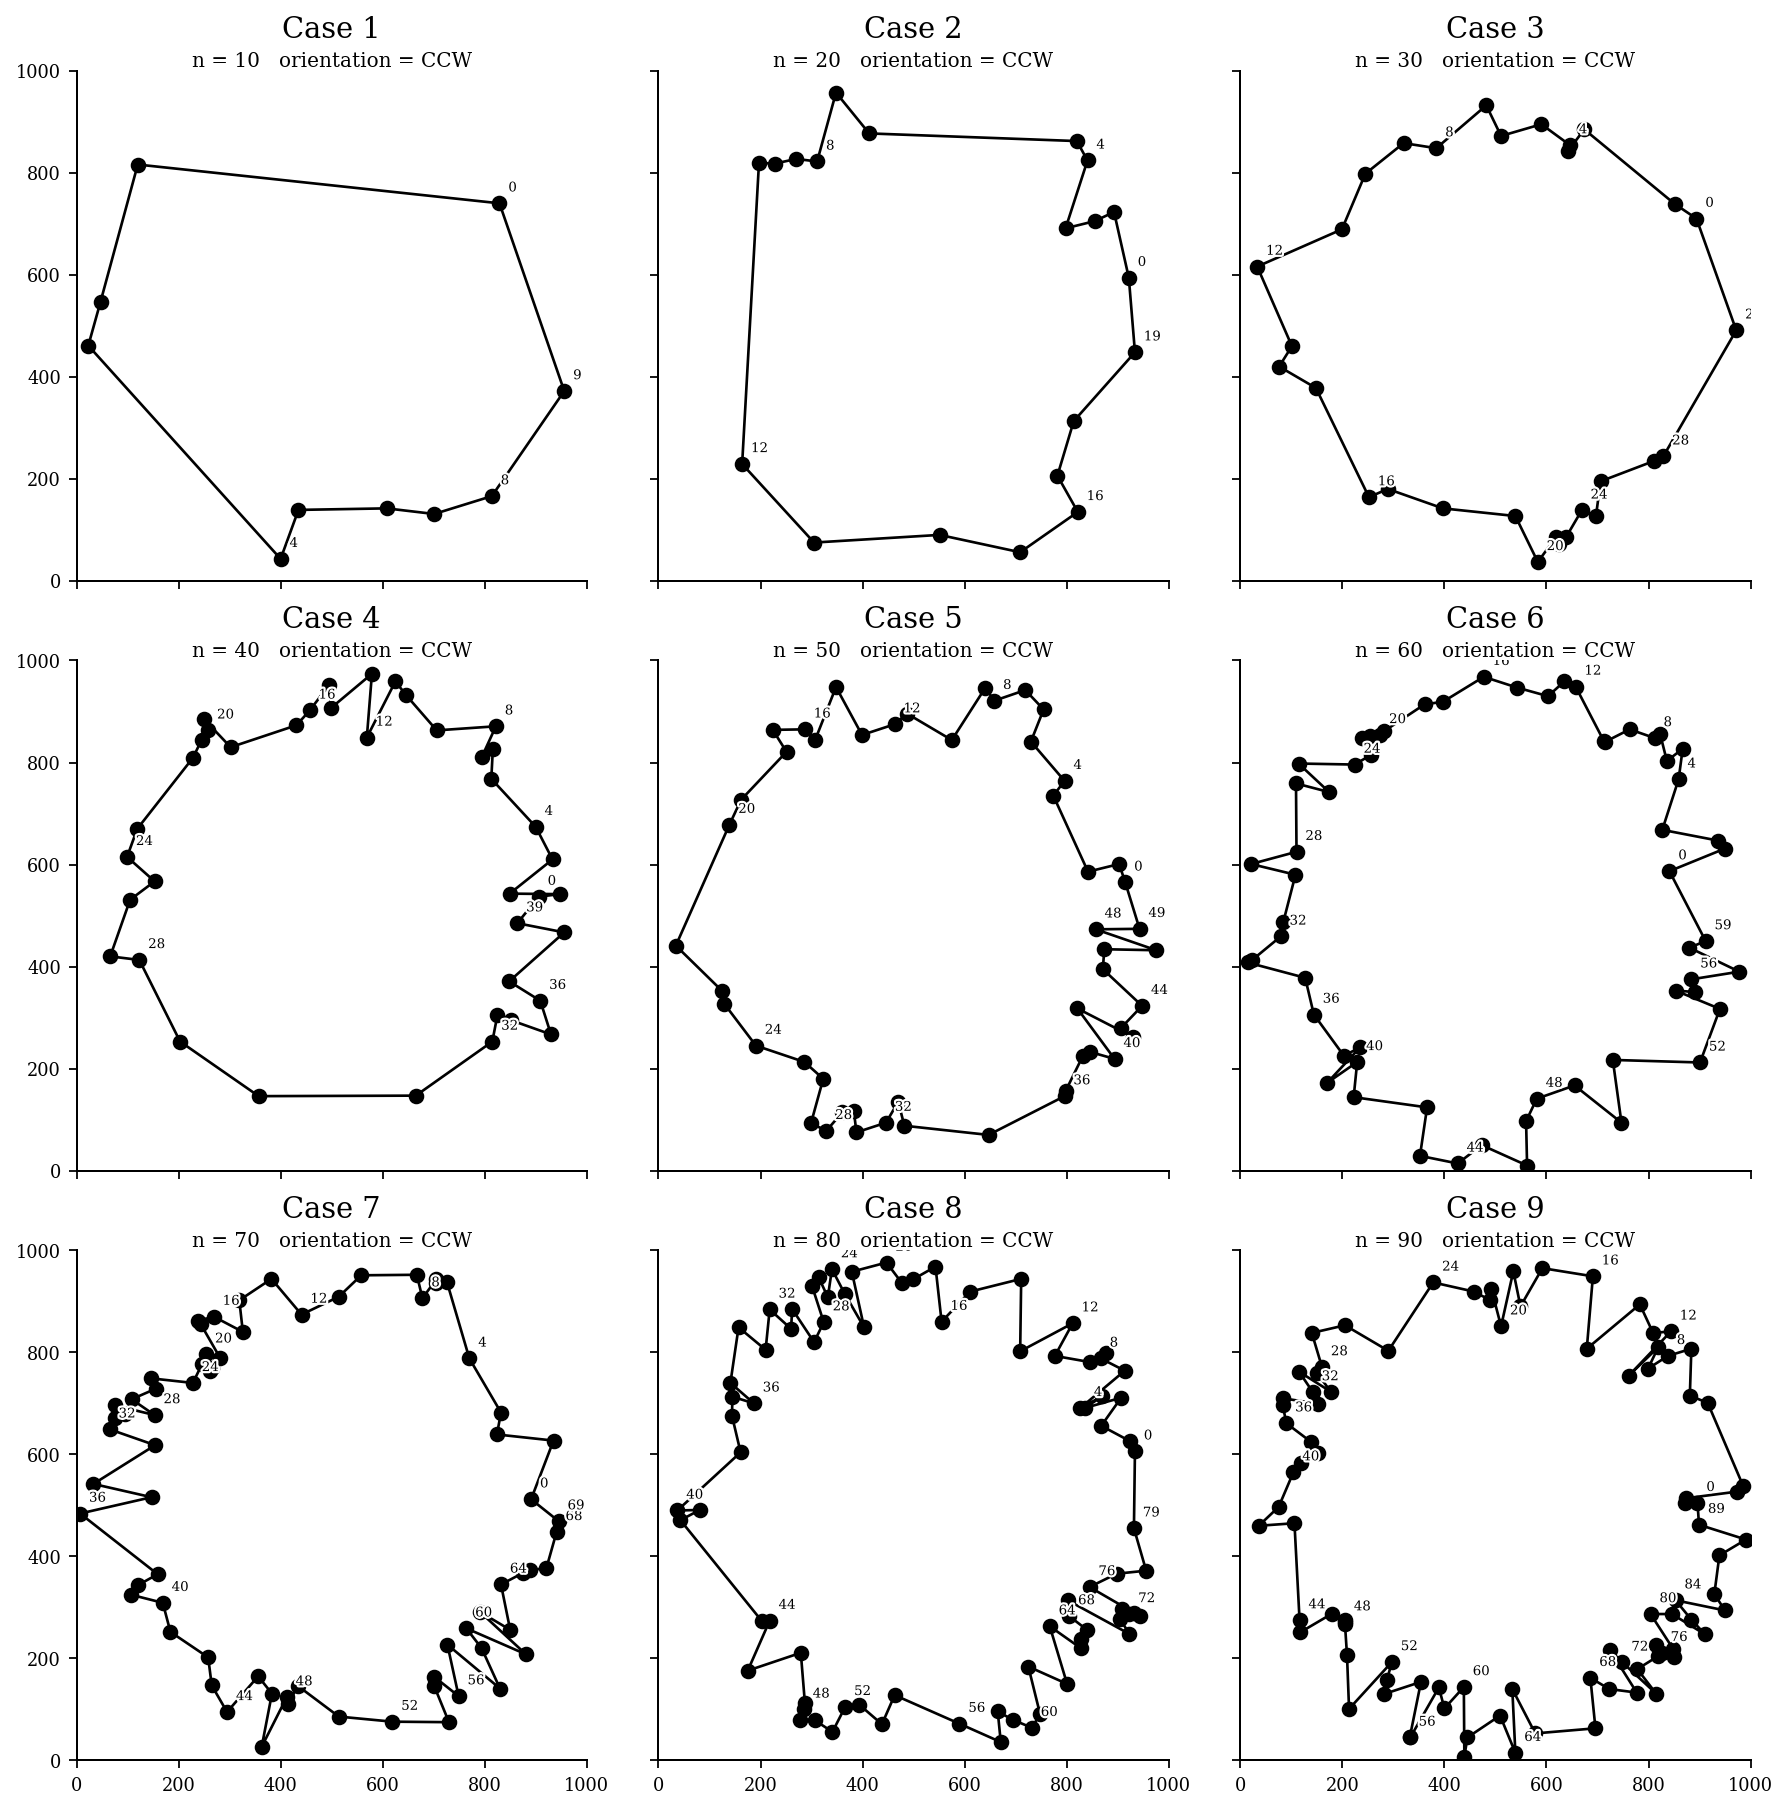
\includegraphics[width=0.95\linewidth]{Pictures/test_polygon_cases.png}
    \caption{Generated simple polygon test cases with increasing vertex counts ($n=10$ to $n=90$). 
    Each subfigure represents a distinct input size used for empirical complexity evaluation.}
    \label{fig:testpolys}
\end{figure}

\begin{figure}[H]
    \centering
    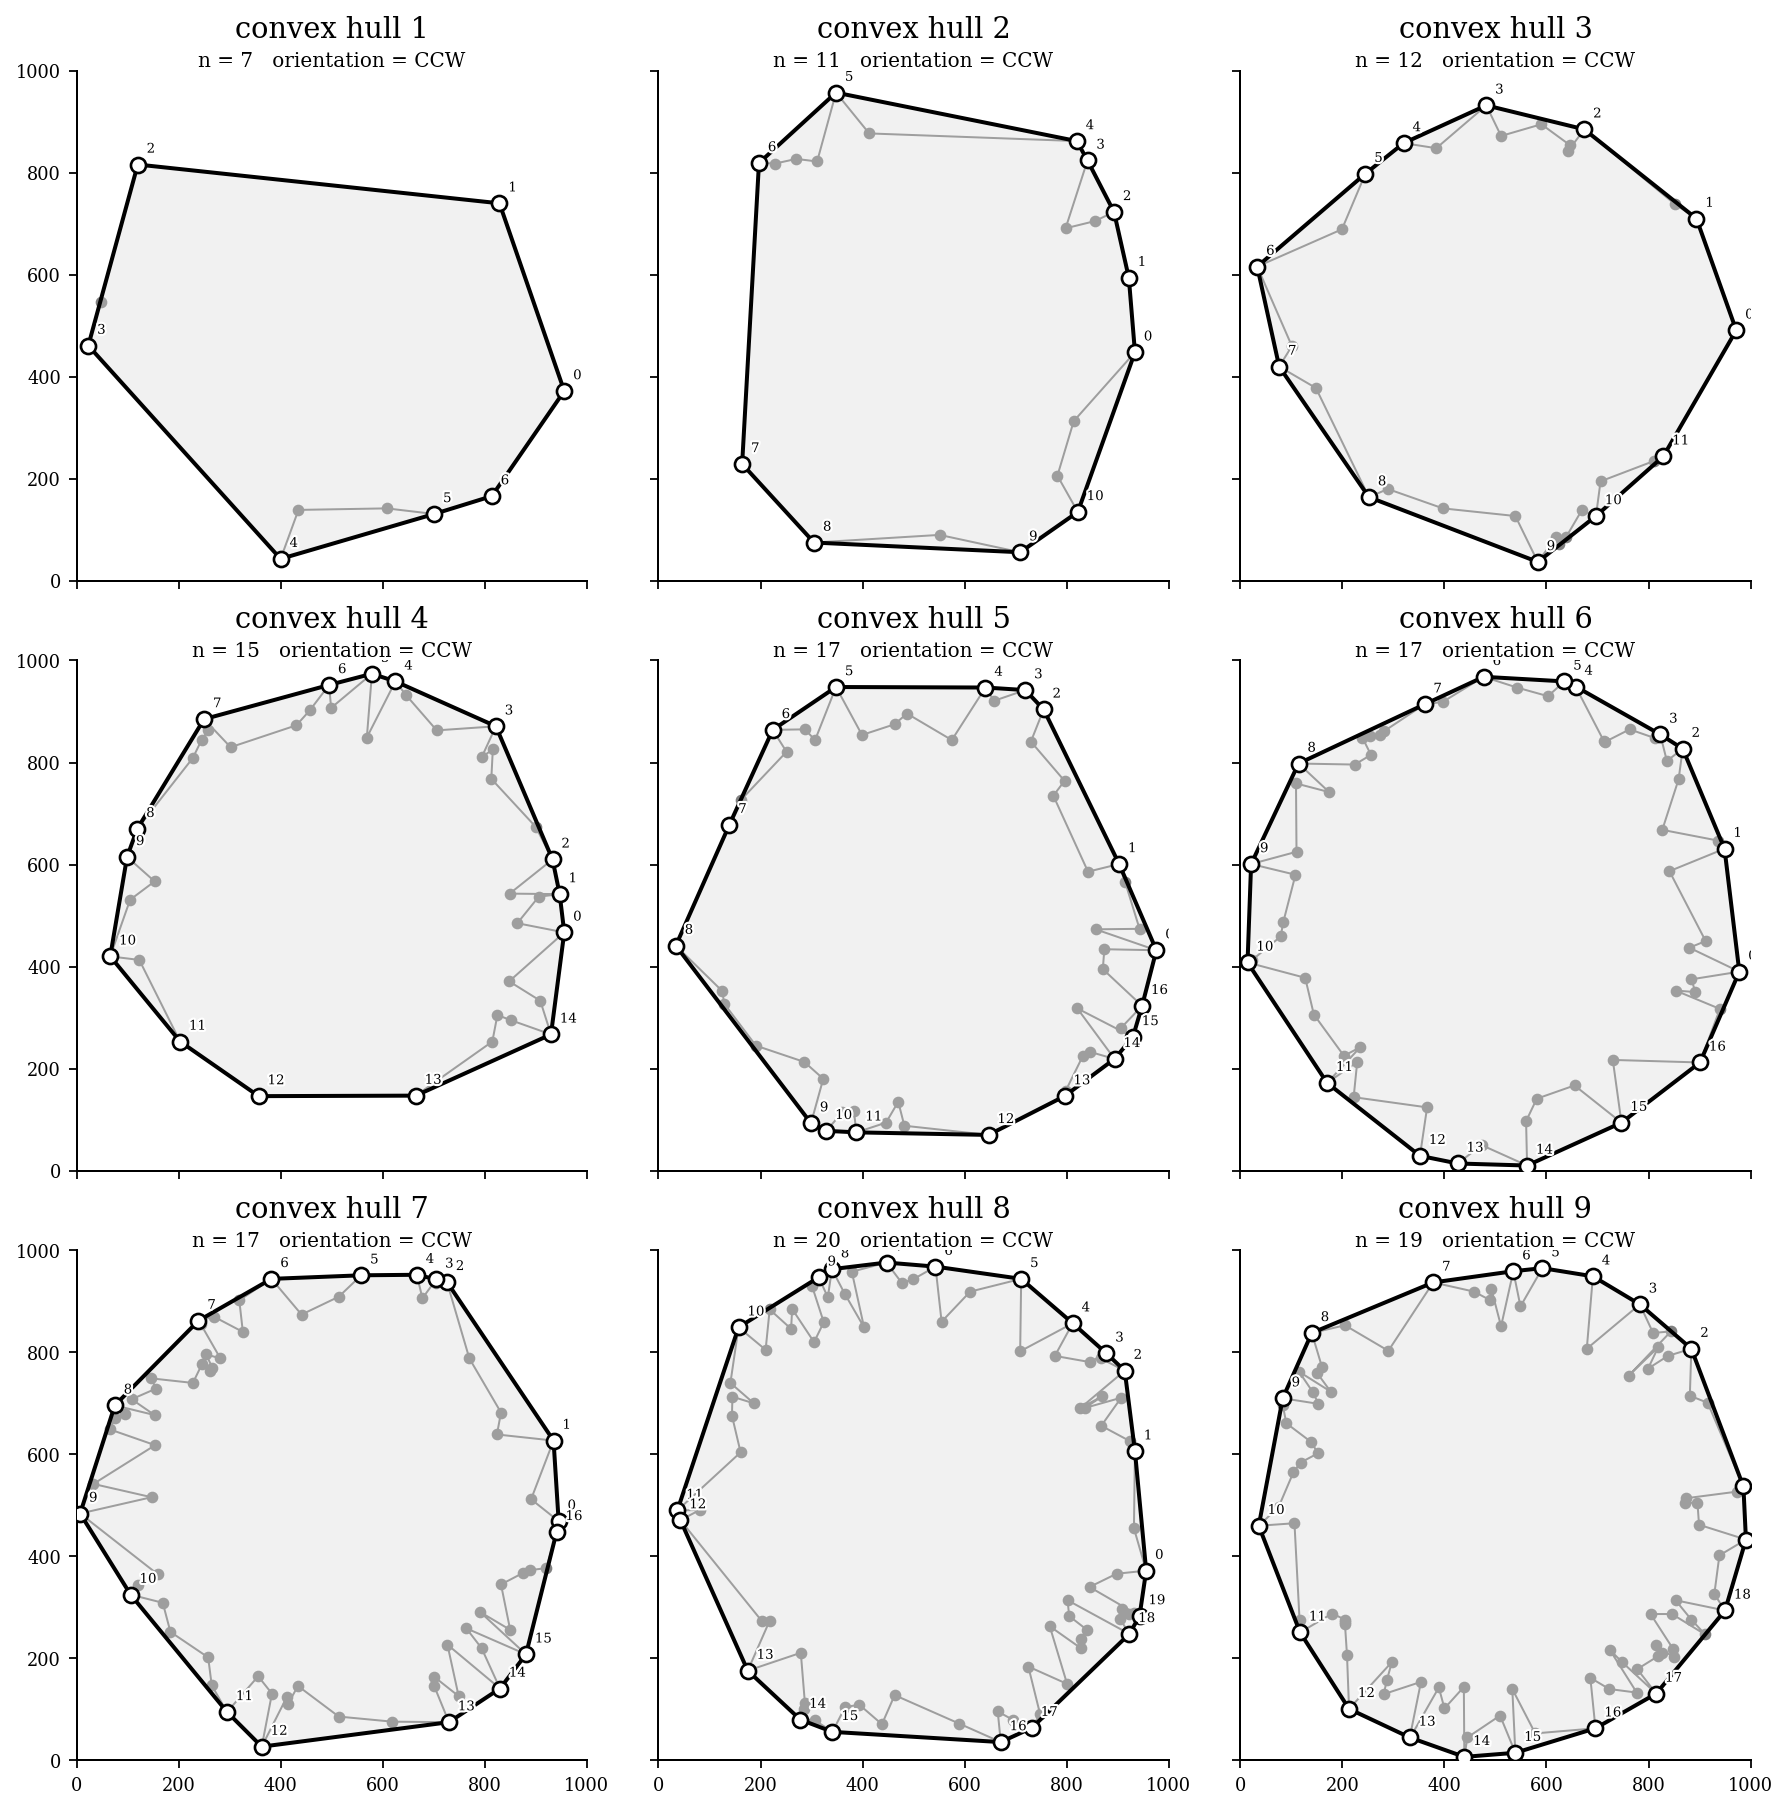
\includegraphics[width=0.95\linewidth]{Pictures/test_hulls.png}
    \caption{Convex hulls computed by Melkman’s algorithm for the test polygons shown in Figure~\ref{fig:testpolys}. 
    The results confirm correctness and stability across all polygon sizes.}
    \label{fig:testhulls}
\end{figure}

After correctness verification, execution time and total operation counts (including orientation, cross-product, and deque operations) were recorded for each test size. 
The results were then fitted to linear and power-law models, as shown in Figure~\ref{fig:complexity}.

\begin{figure}[H]
    \centering
    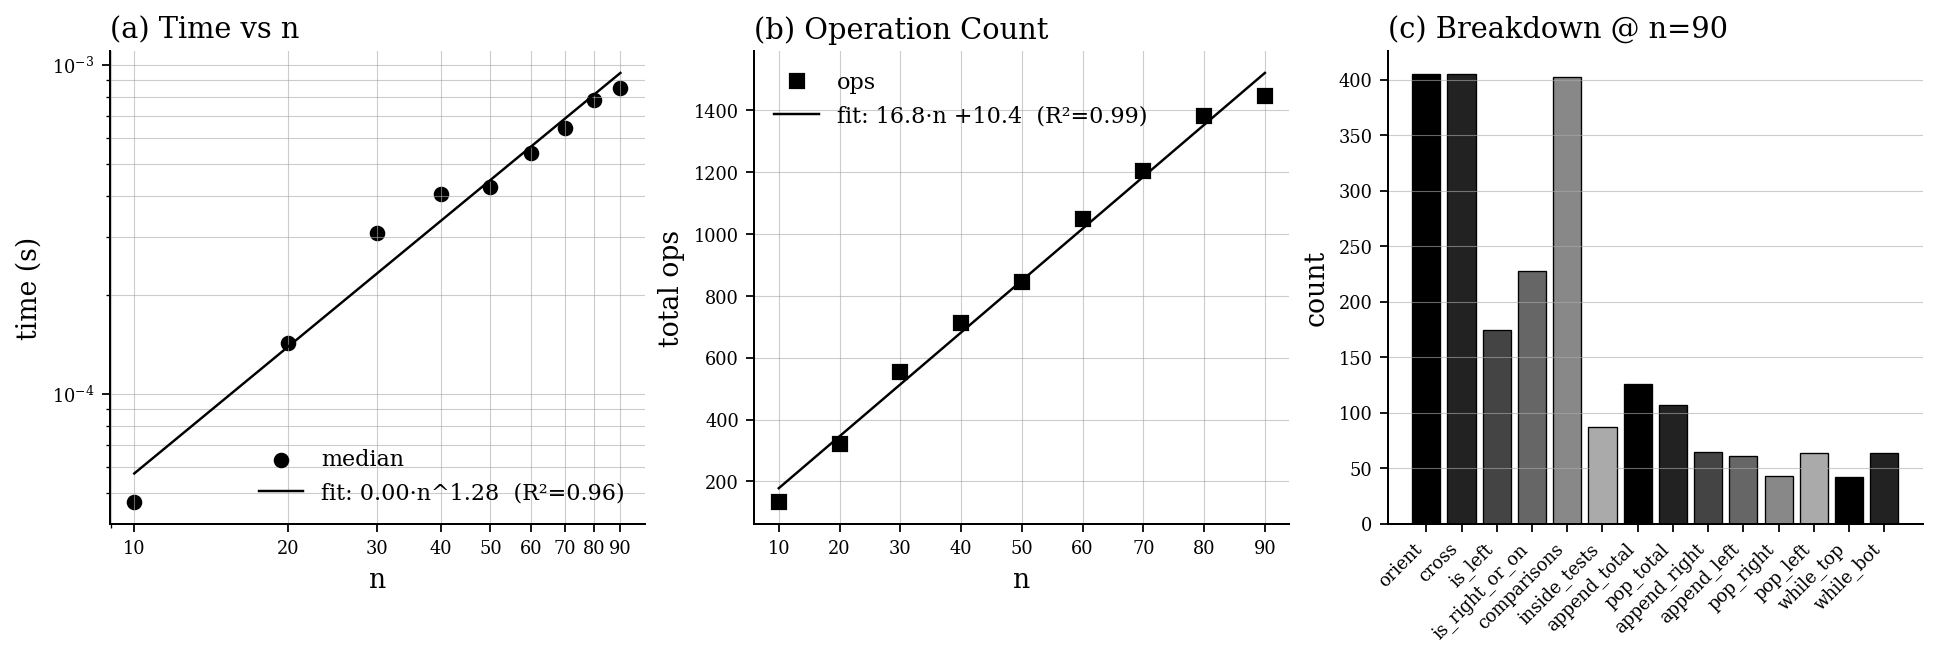
\includegraphics[width=0.95\linewidth]{Pictures/melkman_complexity.png}
    \caption{Empirical complexity analysis of Melkman’s algorithm. 
    (a) Median runtime versus input size $n$, fitted with $T(n)\propto n^{1.28}$ ($R^2=0.96$); 
    (b) total operation count showing a nearly perfect linear fit ($R^2=0.99$); 
    (c) operation breakdown at $n=90$, indicating that orientation and cross-product computations dominate total cost.}
    \label{fig:complexity}
\end{figure}

\textbf{Discussion:}
The measured runtime exhibits an almost linear growth with respect to the number of vertices, with an empirical fit of approximately $T(n)\!\propto\!n^{1.28}$, closely matching the theoretical $\mathcal{O}(n)$ expectation. 
The total operation count maintains a strictly linear relationship with $n$, confirming that each vertex contributes only a constant number of geometric and deque operations. 
The operation breakdown further shows that the majority of computational effort comes from orientation and cross-product evaluations, while deque operations remain minimal.

Overall, the empirical data strongly supports the theoretical claim that Melkman’s convex hull algorithm operates in linear time $\mathcal{O}(n)$, achieving both correctness and computational efficiency across varying input sizes.


\newpage
\problem{General Voronoi}

Study general Voronoi diagrams and implement one variant of your choice.\bigskip

\noindent \textbf{Reference:} Slides of General Voronoi.

\noindent \textbf{Requirements:}
\begin{enumerate}
    \item Explain which variant you chose and why.
    \item Implement the algorithm with proper data structures.
    \item Visualize the result (2D plot showing the sites and Voronoi regions).
    \item Analyze the time and space complexity.
    \item Test cases with at least three different point configurations.
\end{enumerate}

\newpage

\end{document}
